\documentclass{article}
\usepackage[margin=2cm]{geometry}
\usepackage{graphicx}
\usepackage{hyperref}
\usepackage[all]{hypcap}
\usepackage[title,titletoc,toc]{appendix}
\usepackage[english]{babel}
\usepackage[style=authoryear,backend=biber,sorting=nyt,dashed=false,urldate=long,abbreviate=false]{biblatex}
\usepackage{float}
\usepackage{fancyhdr}
\usepackage{microtype}
\graphicspath{ {./images/} }

\setlength{\headheight}{15.2pt}
\pagestyle{fancy}
\lhead{}
\chead{}
\rhead{\bfseries Phase 2 Documentation}
\lfoot{Team Zshell}
\cfoot{COS 301 Software Engineering}
\rfoot{Page \thepage}
\renewcommand{\headrulewidth}{0.4pt}
\renewcommand{\footrulewidth}{0.4pt}

\setlength{\parindent}{0pt}
\setlength{\parskip}{1ex plus 0.5ex minus 0.2ex}

\frenchspacing


\title{
\includegraphics[width=12cm]{Eeufeeslogo.jpg} \\
	\vspace{1.0cm}
	Architectural Requirements Specifications \\ 
	and Design \\
	\vspace{0.5cm}
	NavUP \\
	University of Pretoria \\
	\vspace{0.5cm}
	%\today\\
	\vspace{8.0cm}
	Team Zshell\\
	\vspace{0.5cm}
}

\author{
	Kirker, Timothy\\
	\texttt{u11152402@tuks.co.za}
	\and
	Pritchard, Dawie\\
	\texttt{u13104340@tuks.co.za}
	\and
	Greeff, Claude\\
	\texttt{u13153740@tuks.co.za}
	\and
	Bode, Elizabeth\\
	\texttt{u14310156@tuks.co.za}
	\and
	Suklal, Nicaedin\\
	\texttt{u15207812@tuks.co.za}
	\and
	Magubane, Siyabonga\\
	\texttt{u15289347@tuks.co.za}
	\vspace{0.5cm}
	}

\begin{document}
	\maketitle
	\thispagestyle{empty}
	\clearpage
	
	\newpage
	\pagenumbering{arabic}
	\thispagestyle{empty}
	\tableofcontents
	\clearpage
	
	\newpage
	\section{Architecture Requirements}
		\subsection{Quality Requirements}
		 To create a safe working system that will meet all the required specifications of the NavUP project, specific system requirements need to be looked at in depth. The following are the system requirements that need to be considered. Security, reliability, efficiency, maintainability and usability.
		 
		 \subsubsection{Security}
		 Security is concerned with unauthorized access to specific software functions. An important security measure that needs to be satisfied by the NavUP system is the confidentiality of different user level usernames and passwords. Personal usernames will be set by each user, or their student/staff number will be used to log in. Each user will be required to set their own password. Passwords will be required to be more than 7 characters in length to decrease the likely hood of potential hackers hacking passwords successfully. In the case of a forgotten password, a users password may be reset via a link and an email with a One Time Password. If a user has entered the incorrect password more than 3 times, the account should be blocked and the user should be notified for a password reset. Passwords and any related personal information will be encrypted and safely stored in a 'Users' database.
		 
		  Specific locations will be linked to each user profile. Security will be put in place to allow only that user or other users whom the location is shared with to see the pinned location. Access to the NavUP system will only be made available through the University of Pretoria's firewall network. The firewall will hold as a barrier to deny any outside activity. As different levels of user exist each user will have a specific degree of authority. Admin users will be able to add and remove locations, venues and more permanent locations that will effect the map of the NavUP database. Admin users will have the power to remove lower priority users unwanted actions.
		 
		\subsubsection{Reliability}
		Concerned with the level of risk and chance of application failure. To increase reliability, downtime needs to be reduced and prevented as well as application errors affecting users. Users will need to be navigated to specific locations for classes, practicals and crucial meetings. User authority needs to be kept in place, not allowing users access to prohibited functions allowing them to make unwanted changes to the NavUP system. The NavUP system will need the ability to recover from a failed state, bring back the system to full operation. Finally the NavUP application should withstand any environmental threats that have the potential to cause system failure.
		 
		\subsubsection{Efficiency}
		The two primary sub characteristics of efficiency are broken down into, time behavior and resource behavior. The performance of the NavUP application will be a reflection of how efficient the resources have been used within the application. This will have an effect on the battery life of mobile devices as they are engineered to have a longer life with less processing being done.
		By making use of a microservice architecture we will develop a suite of independent and deployable software services, structuring each non-functional requirement into logical, coherent modules, utilizing the correct design patterns and designs, resulting in maximum efficiency.
		
		\subsubsection{Maintainability}
		As previously mention, each non-functional requirement will be structured logically, enabling future programmers to understand and make necessary changes without the headache of trying to figure out what each code service's purpose is. Due to each software service being independent it will allow code to be worked on without total service down time, this too will contribute to the overall stability, testability and analyzability in identifying the root cause of a failure within the application software.
		
		\subsubsection{Usability}
		The usability is of utmost importance, as we will have a variety of users making use of the NavUP application. Users will range from individuals who are experts at using mobile devices to older generation users who might not be as experienced in using mobiles devices and applications. Features and functions will be easy to understand and use maximizing user experience and making it easy for new users to learn how the application functions.		
	
	\section{Architecture Constraints}
	Constraints are a result of design decisions that are fixed and may not be altered. Constraints may be intentional or unintentional often provided by stakeholders committed toward the project.
		
		\subsection{Programming Language Constraints}
			\begin{itemize}
 				\item Web Based Development
 				\bigskip
 				\\ 				
 				We will be making us of Ionic and Cardova, in which Ionic builds on top of Cardova. By using Cardova, it will take care of packaging the HTML application as a native application that is able to run on Android , iOS and other platforms.
				
				Ionic provides the 'missing peice' as it provides a set of front-end components that allows us to write a HTML application that looks like a native application. These front-end components include (HTML/CSS/JavaScript and AngularJS).
 				
  				\item Server Side Development
  				\bigskip
				\\
 				User information, information regarding locations and venues will be stored within a database. To run the database we will make use of mySQL and PHP and AJAX, where validation will be done by PHP.
 				
 				\item Mobile Application  Development
  				\bigskip
 				\\
 				The mobile application will be built using Android Studio (Java).
 							
			\end{itemize}


		\subsection{Operating System Constraints}			   
 				The NavUP application needs to run on Windows, iOS and Android at the very least. Building software that fails to satisfy the platform constraint means we have failed to deliver what is expected by the external stakeholder. 
 				
 		\subsection{Network Constraints}			 
 				The NavUP application will run on the Universities network allowing only users within the firewall to make use of the application.
 				
 	\pagebreak
 	
	\section{External Interface Requirements}
	
	\subsection{User Interfaces}

The NavUP application will consist of different user interfaces, depending on the user's level of authority. Each level of UI will be appropriate with 
regards to the ease of use. The 'Guest' users with the lowest level of authority with have a basic, easy to use view. Guest users will be new to using
the NavUP application and assistance will be prompted to guide the user through all the available features. The application UI will be so that
new users are able to use it as well as to satisfy experienced users.


Admin users and Lecturers with higher levels of authority will have a variety of added features added to their UI. The ability to add events, venues and
locations would be satisfied by a more detailed UI. These users will also be able to make permanent changes to the NavUP database as well as make changes
to lower level user's information.


Visually the UI of all users will cater for people with disabilities with a easy to read and understand layout.
.	
	\subsection{Hardware Interfaces}
	
	The NavUP application will be a web and mobile compatible application. Focusing on the mobile side of things, the application will be able to run on any
device which runs on Android or iOS. The software will be written in the most efficient way as possible to put as little stress on the CPU as possible
allowing for longer battery life. The application does not write directly to the users device but instead to the NavUP database which is located on a 
network server. Users will have to be within the network firewall of the University of Pretoria to make use of the NavUP application. The user's device
transfers and receives data from the server using a set of secure network protocols ensuring information is not compromised.

	\subsection{Software Interfaces}	

As mentioned the application will run on Android and iOS. On the server side, the servers can either make use of Windows,Linux or UNIX, but it is required
to have MySQL installed and configured.
	
	\subsection{Communications Interfaces}
	
Data and information between users and servers will communicate through the network of the university.

	\pagebreak
 	\section{Architectural Patterns or Styles}
 	We will be implementing the microservices architectural pattern. As well as different architectural patterns for each subsystem
 	
 		\subsection{Benefits}
 			\begin{itemize}
 				\item Deployability
 				\bigskip
 				\\
 				Redeployment is not necessary when changes are made to code preventing the risk of disruption.
 				Developers are able to deploy independent services without having to wait on others to complete their modules, this improves time management and contributes to the overall flexibility.
 				\item Changeability
 				\bigskip
 				\\
 				Due to constant changes in technologies and user requirements upgrades need to be made to adapt to these new changes. Microservices  facilitate this very well allowing independent services to be upgraded.
 				\item Ability to Utilize Different Technologies
 				\bigskip
 				\\
 				Java may be used for event processing microservices due to multithreading properties of JVM.
 				This allows programmers to make use of new technologies on services without disrupting of causing system failure.
 				\item System Resilience
 				\bigskip
 				\\
 				If a microservice stops working, only small, very specific functionality will be lost. This enables programmers to build resilience by making use of smaller independent services.
 			\end{itemize}
 		\subsection{Concerns}
 			\begin{itemize}
 				\item Complexity
 				\bigskip
 				\\
 			\end{itemize}
 			 \section{Architectural Patterns for subsystems}
				\subsection{User Subsystem}
				For the User module we will be using a layered architecture, allowing the use of dependency injection allowing for pluggable application architectures
					\subsubsection{Benefits}
 						\begin{itemize}
 							\item Seperation of Concerns
 							\bigskip
 							\\
 							Seperates the business logic from the presentation, thus allowing you to work on seperate layers independently, allowing non-repeatability
 							\item Flexibility
 							\bigskip
 							\\
 							Coping with growth or traffic will be easier to handle.
 							\item Each layer can evolve independently
 							\bigskip
 							\\
 							Since each layer is independent from each other, each layer will be able to change without affecting any of the other layers.
 							\item proven and stable protocols and design
 							\bigskip
 							\\
 							 One of the most commonly used architectures means that protocols and designs means the system will be stable.
 						\end{itemize} 
	\subsubsection{Concerns}
 			
 				There are many problems that can occur but the main one would be how to design the application so that it supports maintainability, extensibility, security and scalability.
 	\subsubsection{External Interface Requirements}
	 	These requirements outline the external interfaces needed in terms of hardware, software and GUI For the users module.
	 	\begin{itemize}	 		
	 	\item \textbf{User Interfaces:}
	 	\\The system will make use of of  ionic and cordova, which is a cross platform user interface that will support windows, IOS and android. The reasoning is that the application has to work on multiple platforms, this enables us to use one specific technology for the user interface.
	 	
	 	\item \textbf{Hardware Interfaces:}
	 	\\The hardware interfaces will only be hardware where the application can run on. The four hardware interfaces that will be used will be a Personal Computer, a laptop, a mobile phone and a tablet.
	 	
	 	\item \textbf{Software Interfaces:}
	 	\\The users module will have different interfaces for each section of a layered architecture. The presentation layer will make use of Tabris. The business layer will use java EE's REST API.  The persistence layer will use JPA and the database layer will make use of JDBC and that database will be done via PostgreSQL. All of these interfaces make use of Java EE as to make it easier for dependency injection.
	 	
	 	\item \textbf{Platform Considerations:}
	 	\\The application will make use of windows, Android and IOS. The hardware and software must be able to support each platform and work independently from one another.
	 \end{itemize}
	 
 	\subsubsection{Performance Requirements}
 	These Requirements outline what navUP should be able to maintain during the course of its lifetime in terms of the performance of the application
 	\begin{itemize}
 	\item \textbf{Response Time:}
 \\	The system warrants that even if over 40 000 students are connected. The performance of the application will not fall under 10 seconds of waiting a response from the application. This includes on each platform(IOS,Android, Windows). This also includes the infrastructure of the application, as well as front - ends. The response time will be measured using filters within Java EE. 
 	
 	\item \textbf{Workload:}
 	\\The application must support all the students on UP campus( around 40 000), as well as guests and administrators of the application in which 15 000 will use the application on a day to day basis.
 	In terms of login. around 90 percent of active users will log in and log out of the application each day. In terms of public services around 70 percent will use them each day. In terms of administrators. Changes will be made around 60 percent each day.
 	\item \textbf{Scalability:}
 	\\The application will be capable of supporting at least users each day. As long as the application is implemented in such a way as to support large amounts of users.
 	
 	\item \textbf{Platform Considerations:}
 	\\The application will make use of windows, Android and IOS. The hardware and software must be able to support each platform and work independently from one another.
 \end{itemize}
 	
 	\subsubsection{Design Constraints}
 	These Requirements outline what navUP should be able designed according to the client.
 	\begin{itemize}
 		\item Modularity:
 		Each activiity of the system is done by exactly one module. 
 		
 		\item Minimal Dependency:
 		The use of dependency injection to make sure modules are as loosely coupled as possible, In a layered architecture. Making sure layers are also loosely coupled.
 		
 		\item Well Defined Input:
 		Every input/output is needed for the function of that specific module.
 		
 		\item Abstraction:
 		Make sure changes later wont affect the application as a whole, by abstracting the implementation details.
 	\end{itemize}
 	
 	\subsubsection{Software System Attributes}
 	\begin{itemize}
 		\item \textbf{Security:}
 		\\Users or guests are not allowed to alter fields in the database. This will be done through prepared statements in JDBC.
 		
 		\item \textbf{Flexibility:}
 		\\The architecture is designed in such a way that any layer  may be altered without changing any other layer. Thus to adapt those layers becomes increasingly easy.
 		
 		\item \textbf{Maintainability:}
 		\\By the use of a layered architecture the system will remain easy to maintain since we will be using common tested methods to make it easy to fix bugs, and improve the system over time due to the loosely coupled nature of a layered architecture.
 		
 		\item \textbf{Availability:}
 		\\If one layer fails, since a layered architecture is loosely coupled. The application will be available most of the time. Since a failure on one layer will not completely break the database or application in any way.
 		
 		\item \textbf{Efficiency:}
 		\\The database will be accessed accordingly and through the use of JDBC and RESTful webservices, the required processing will be done in the least amount of time with the least amount of hardware.
 		
 		\item \textbf{Resilience:}
 		\\The application will handle heavy loads due to the fast processing nature of a layered- architecture.
 		
 		\item \textbf{Modularity}
 		\\The user module is broken up into layers, each layer is a seperate component which can be worked on independently.
 	\end{itemize}
			
	\subsubsection{Design of the Architecture}
		\begin{itemize}
 				\item Class Diagram
 				\begin{center}
					\begin{figure}[!h]
					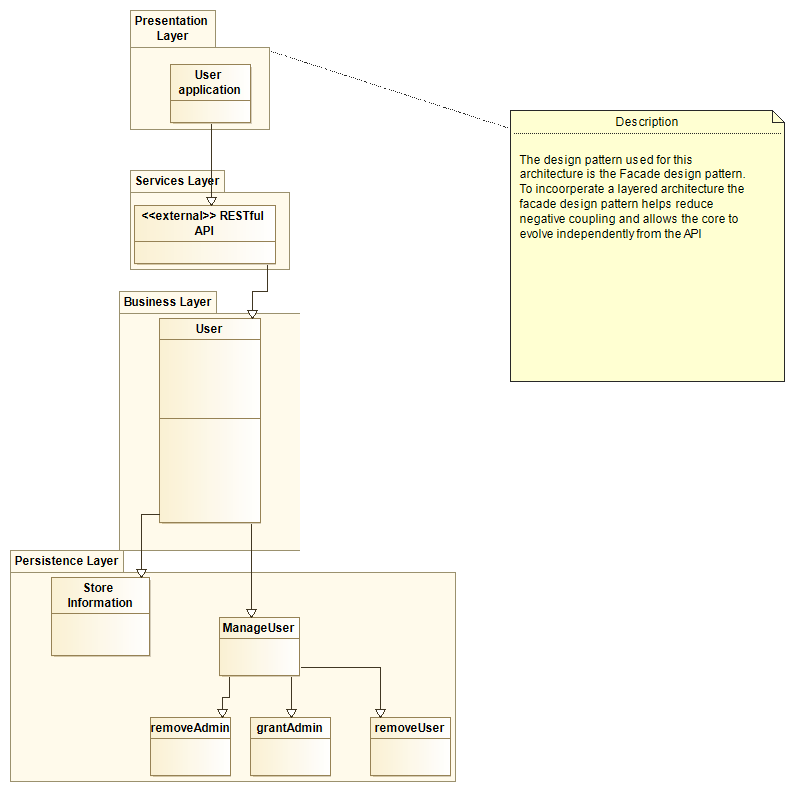
\includegraphics[scale=0.5]{cdu.png}
					\caption{User Module Class Diagram}
					\end{figure}
				\end{center}
	 			\clearpage
	 			
	 			\item Deployment Diagram				
	 			\begin{center}
	 				\begin{figure}[!h]
	 					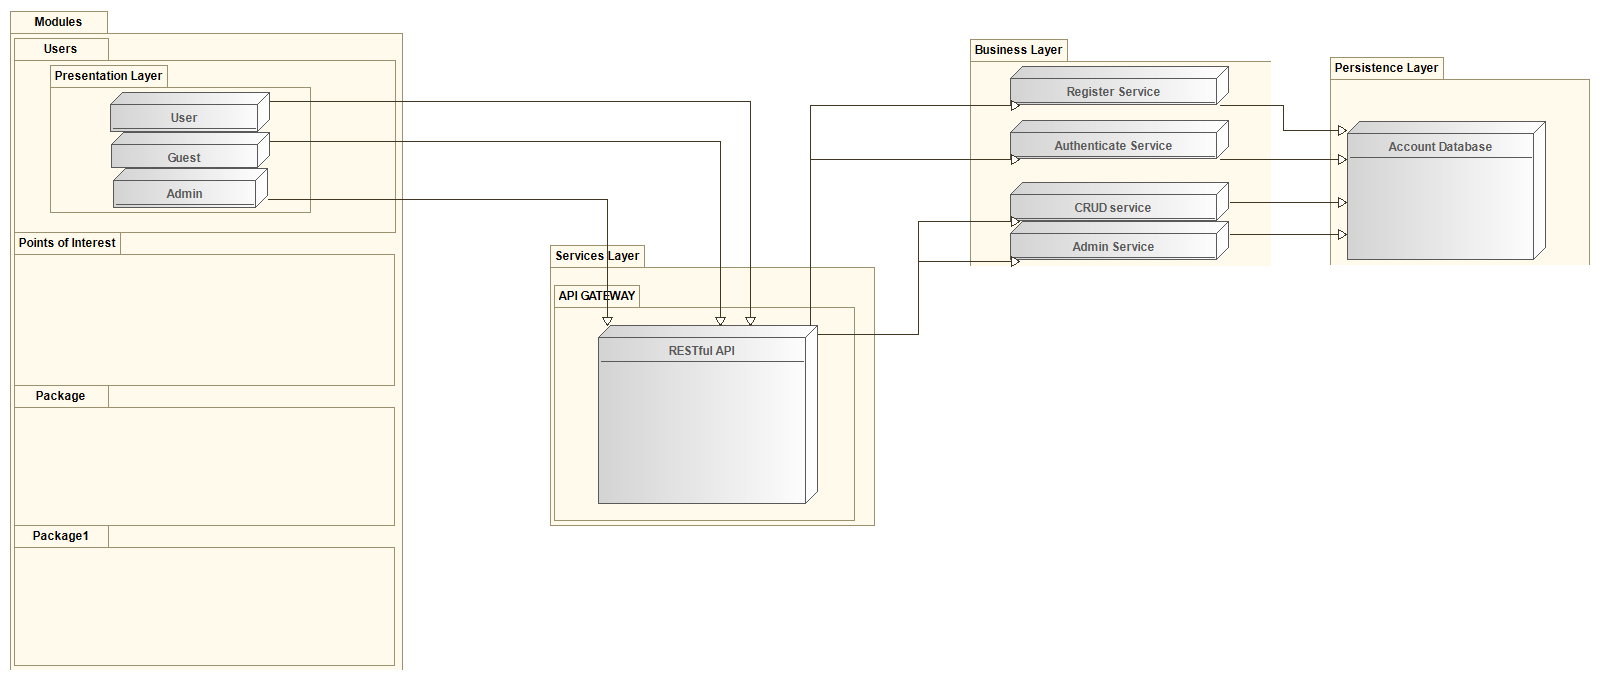
\includegraphics[scale=0.3]{dd.png}
	 					\caption{User Module Deployment Diagram}
	 				\end{figure}
	 			\end{center}
	 			
	 			\item Use Case Diagram
	 			\begin{center}
	 				\begin{figure}[!h]
	 					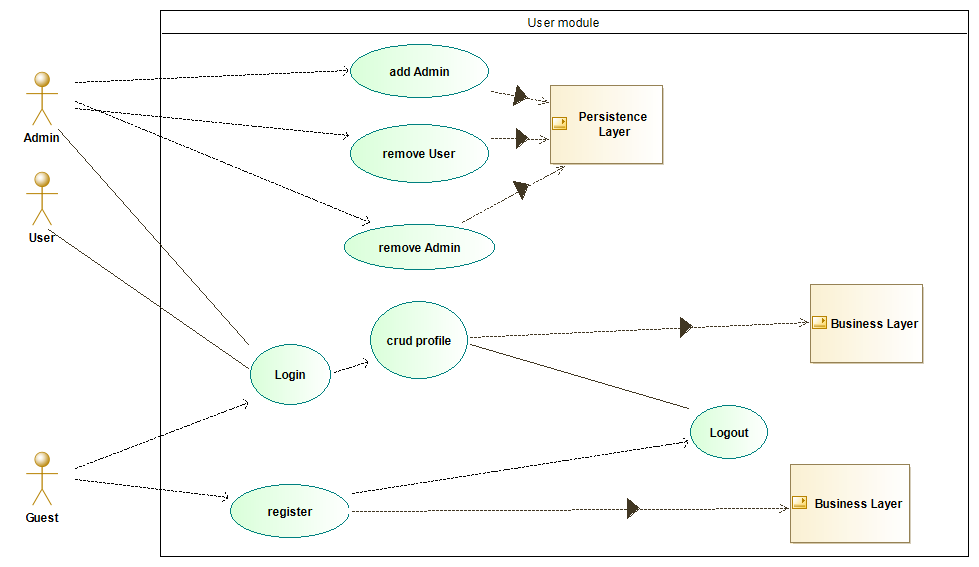
\includegraphics[scale=0.5]{uuc.png}
	 					\caption{User Module Use Case Diagram}
	 				\end{figure}
	 			\end{center}
	 			\pagebreak
	 			
				\item Sequence Diagram				
 				\begin{center}
 					\begin{figure}[!h]
 						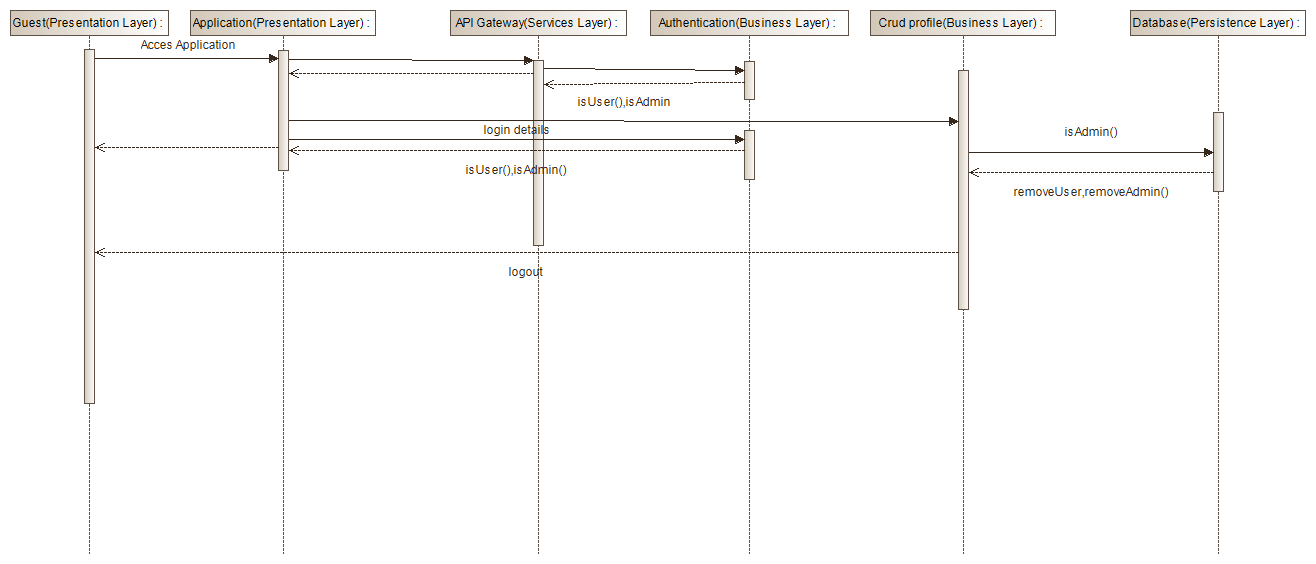
\includegraphics[scale=0.4]{isdu.png}
 						\caption{User Module Sequence Diagram}
 					\end{figure}
 				\end{center}
 				
 				\item Activity Diagram
 				\begin{center}
 					\begin{figure}[!h]
 						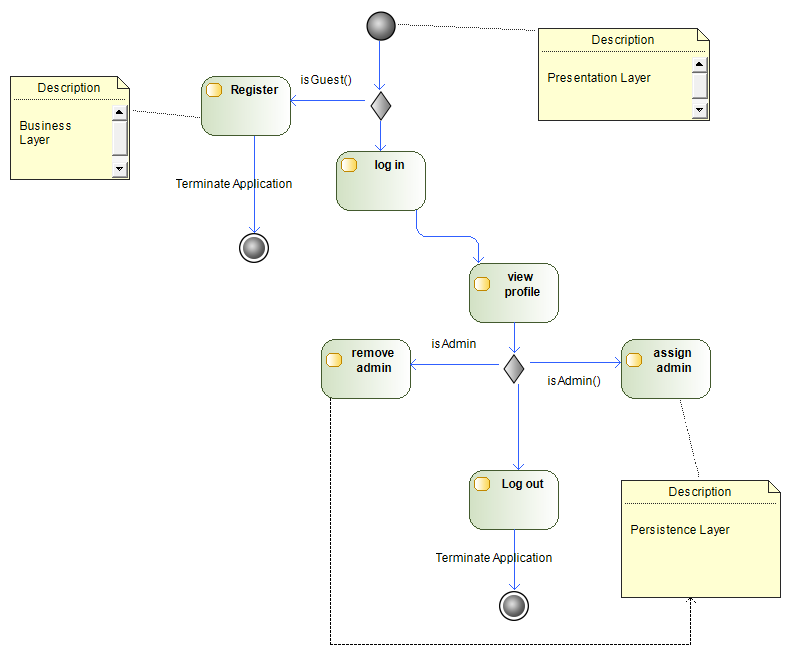
\includegraphics[scale=0.4]{uad.png}
 						\caption{User Module Activity Diagram}
 					\end{figure}
 				\end{center}
 				\pagebreak
 				
				\item State Diagram
				\begin{center}
					\begin{figure}[!h]
						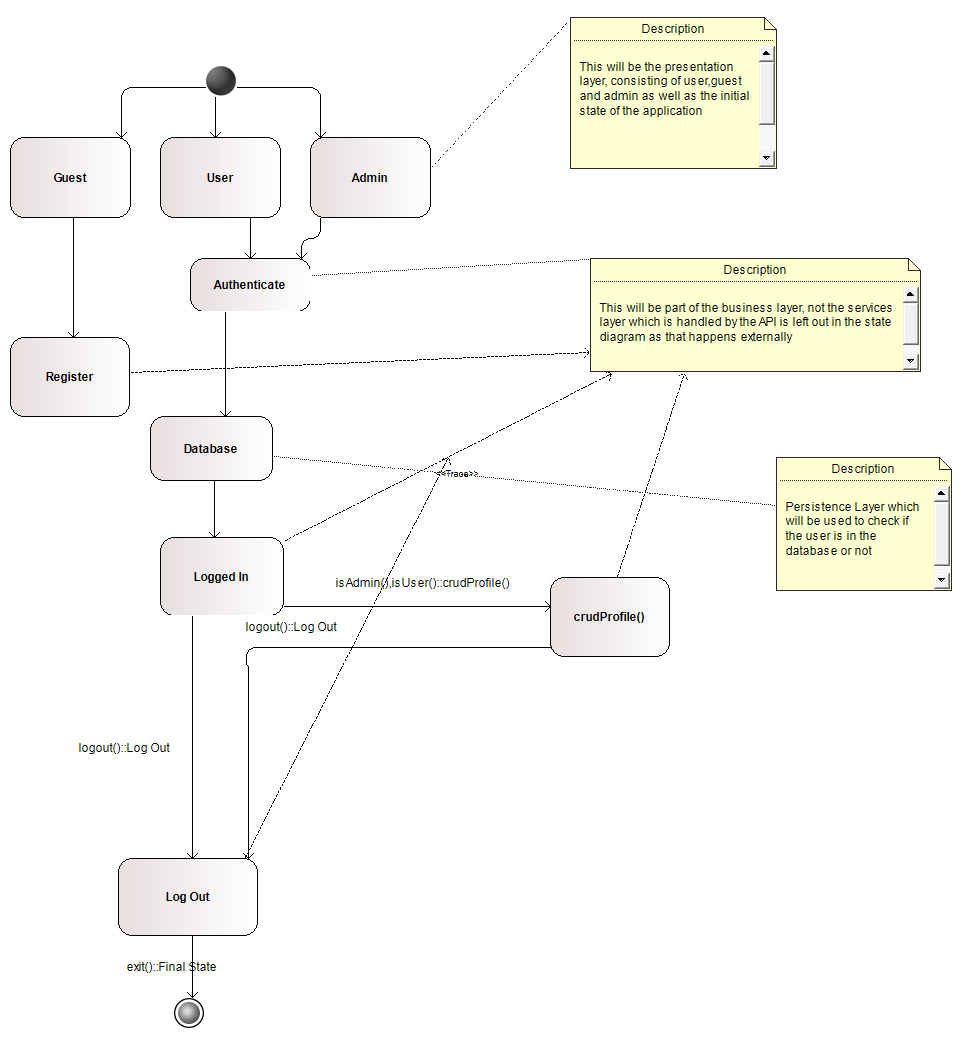
\includegraphics[scale=0.5]{smdu.png}
						\caption{User Module State Diagram}
					\end{figure}
				\end{center}
			
 		\end{itemize}
	\subsubsection{Technologies}
			\begin{itemize}
 				\item Presentation Layer
				\\
				\\
				For the presentation layer we will use android studio as well as iOS and Web front end. This is to make the application available on multiple platforms which is important
 			
				
 			
				\item Business Layer
				\\
				\\
				For the business layer we will use Java Enterprise Editions' REST API, this is for improved scalability since the client and server are loosely coupled.
 				
			
 				\item Persistence Layer
				\\
				\\
				For the Persistence layer we will use Java Persistence API(JPA), for accessing, managing and persisting data between data transfer objects. This allows us to focus more on the object model than the actual SQL, enables us to save time by generating/updating SQL queries and convert the results to our model classes.
	
				
				\item Database Layer
				\\
				\\
				For the Database layer we will use JDBC, which offers a natural java interface therby making it easier to work with SQL, this works well since our persistence layer is generating SQL queries for u, allowing us to manage and manipulate the database.
				
			
 		\end{itemize}
 		
 		\subsection{Navigation Subsystem}
 		\subsubsection{Type of System and Architecture Design}
				For the implementation of the Navigation module the well known design pattern 'Facade' has been used within a layered architecture. The reasoning behind the use of this design pattern is creating a simpler interface to a underlying complex system. This will contribute to easier maintainability by making the use and testing of the code easier for the software developer. It will also reduce dependencies of outside code on the inner working classes within the Facade design pattern, adding to the flexibility of the overall system. The route management will be within the Persistence layer of the multitier architecture.
				
		\subsubsection{Design of Architecture}
				
			\begin{itemize}
 				\item Class Diagram
 				\begin{center}
 					\begin{figure}[!h]
 						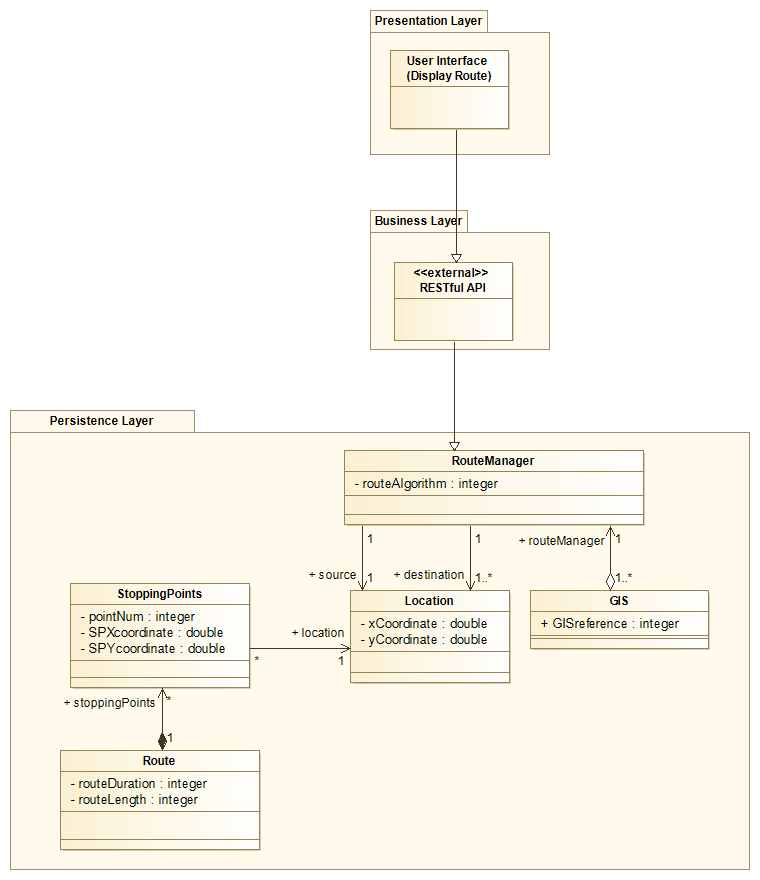
\includegraphics[scale=0.275]{navigationCD.png}
 						\caption{Navigation Module Class Diagram}
 					\end{figure}
 				\end{center}
 				\pagebreak
			
			\item Deployment Diagram
			\begin{center}
				\begin{figure}[!h]
					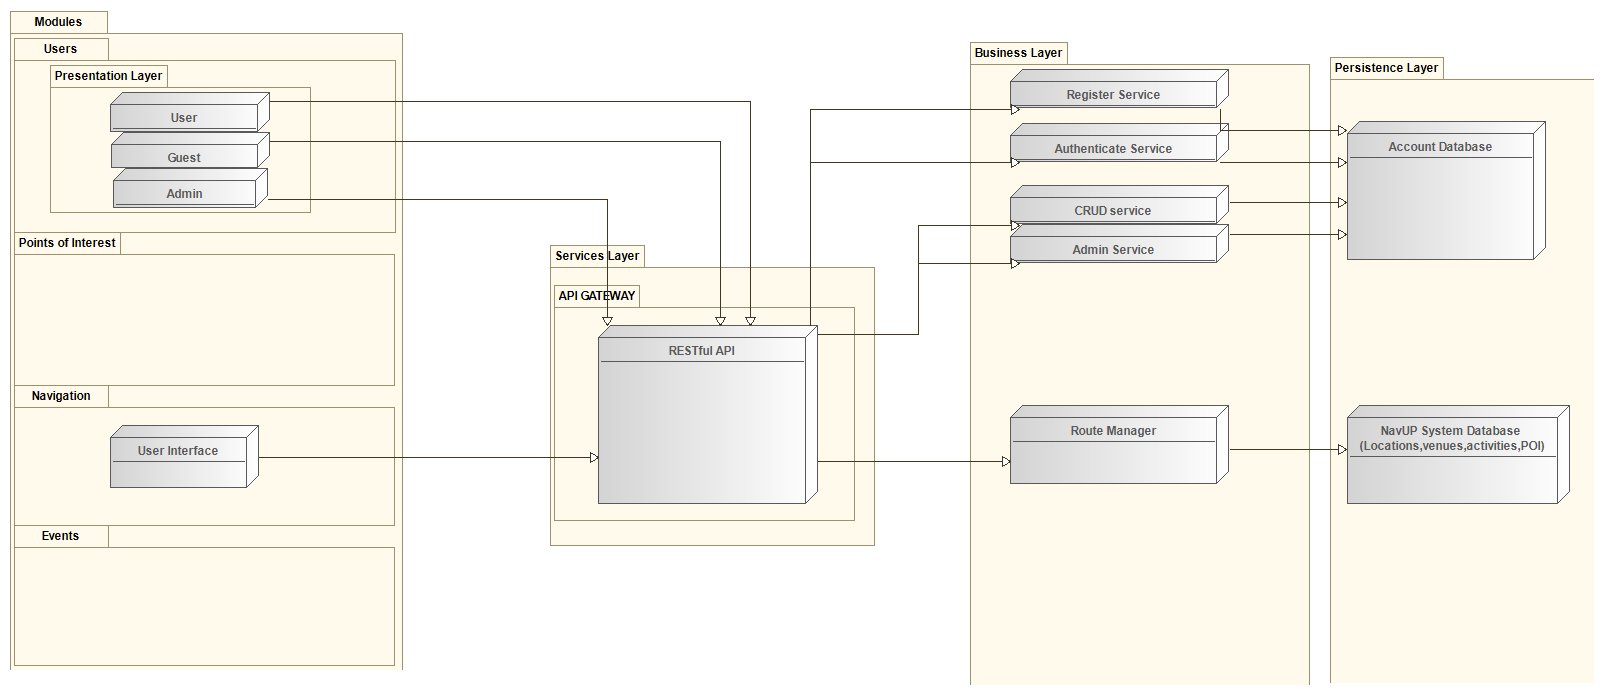
\includegraphics[angle=90, scale=0.35]{navigationDeploymentDiagram.png}
					\caption{Navigation Module Deployment Diagram}
				\end{figure}
			\end{center}
			\pagebreak
			
			\item Use Case Diagram
			\begin{center}
				\begin{figure}[!h]
					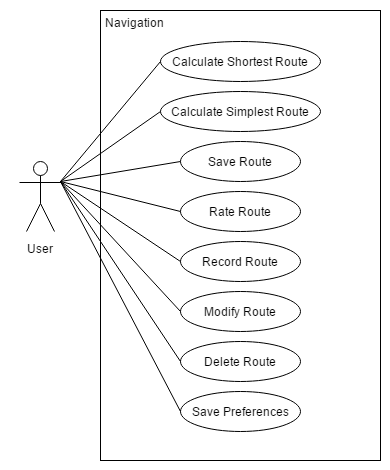
\includegraphics[scale=0.8]{Navigation_Use_Case_Diagram.png}
					\caption{Navigation Module Use Case Diagram}
				\end{figure}
			\end{center}
			\pagebreak
			
				\item Sequence Diagram
 				\begin{center}
 					\begin{figure}[!h]
 						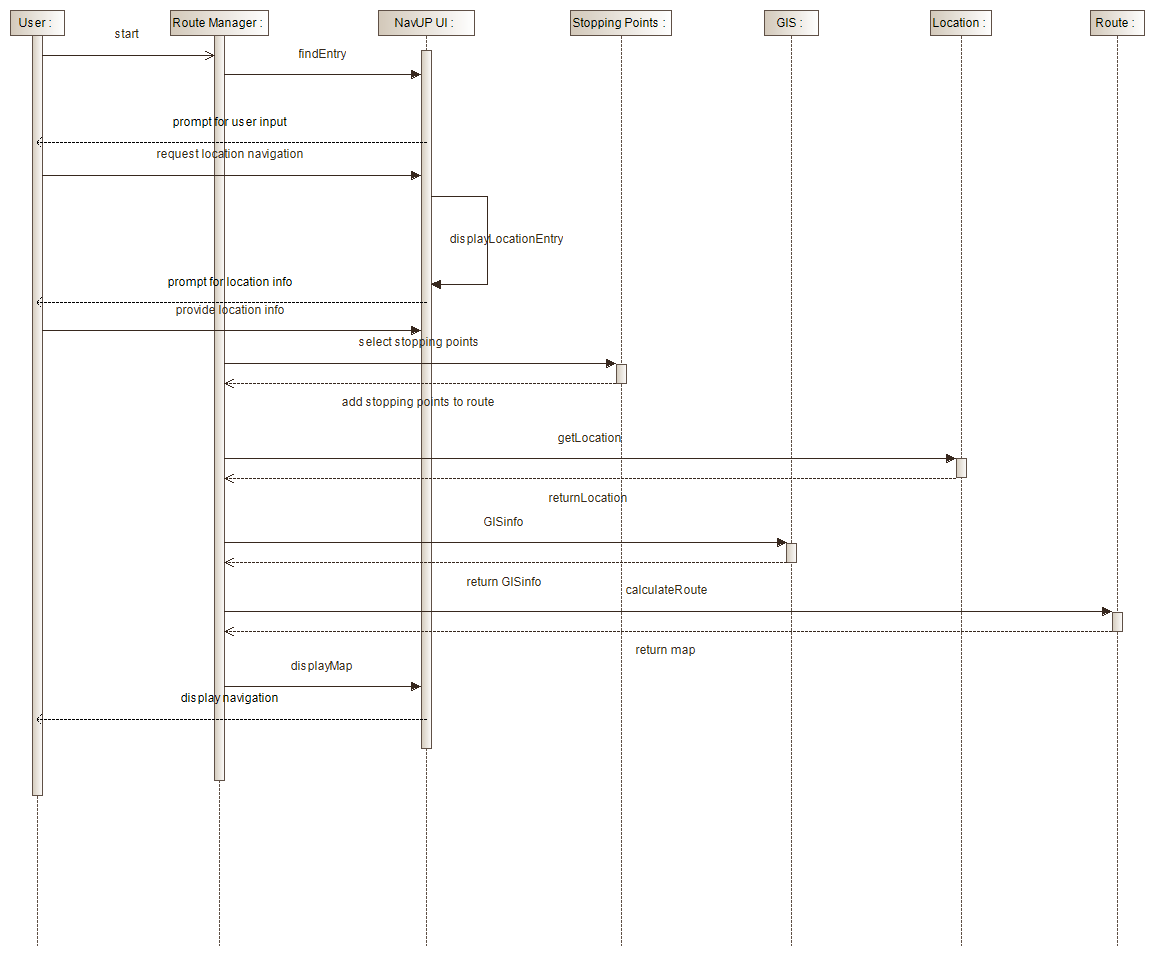
\includegraphics[scale=0.45]{navigationSequenceDiagram.png}
 						\caption{Navigation Module Sequence Diagram}
 					\end{figure}
 				\end{center}
			\pagebreak		
			
				\item Activity Diagram
 				\begin{center}
 					\begin{figure}[!h]
 						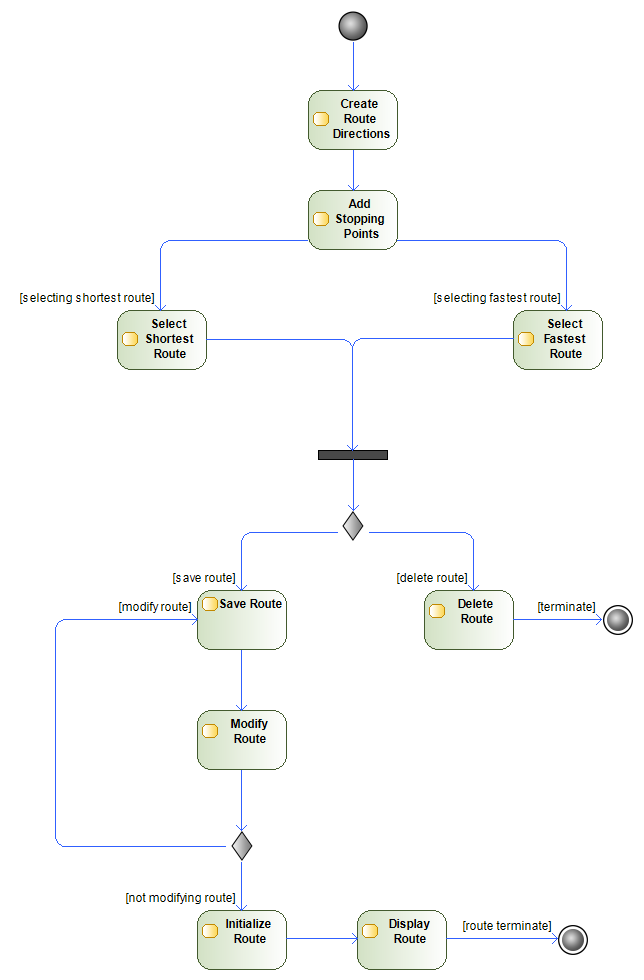
\includegraphics[scale=0.45]{navigationActivityDiagram.png}
 						\caption{Navigation Module Activity Diagram}
 					\end{figure}
 				\end{center}
				
				
			\end{itemize}
		\subsection{Point Of Interest Subsystem}
			
 		\subsubsection{Type of System and Architecture Design}
The POI(Point of Interest) subsystem will be implemented using the N-tier architecture which is structured into the graphic user interface, controller, business objects, database and network communication layers.The POI subsystem is an interactive subsystem that uses predefined protocols namely the GIS module which supplies the information location allowing the POI subsystem to implement the CRUD locations functional requirement: Drop a pin and name it. Show saved pins. Edit detail about pins. Delete pins.The GUI layer is responsible for getting the user’s input into the system for example the admin user. The information is transferred through a controller layer object to the database layer where the network communication layer may be invoked in the event where the database is located in a remote site.

		\subsubsection{Domain Model }
The conceptualization process of the POI will help provide a common conceptual basis for subsequent design, implementation, testing and maintenance.The visualization of the domain model of POI is represented by the following UML diagrams below.



		\subsubsection{Design of Architecture}
			\begin{itemize}
 				\item Class Diagram
 				\begin{center}
 					\begin{figure}[!h]
 						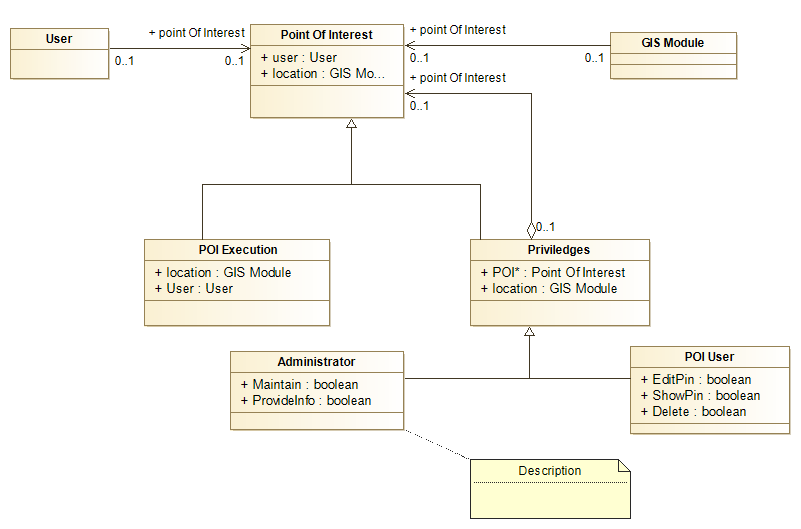
\includegraphics[scale=0.6]{POI_ClassDiagram.png}
 						\caption{Point of Interest Module Class Diagram}
 					\end{figure}
 				\end{center}
			%\pagebreak
			
			\item Deployment Diagram
			\begin{center}
				\begin{figure}[!h]
%					\includegraphics[scale=0.5]{} 
					\caption{Point of Interest Module Deployment Diagram}
				\end{figure}
			\end{center} 
			\pagebreak
			
				\item Use Case Diagram
 				\begin{center}
 					\begin{figure}[!h]
 						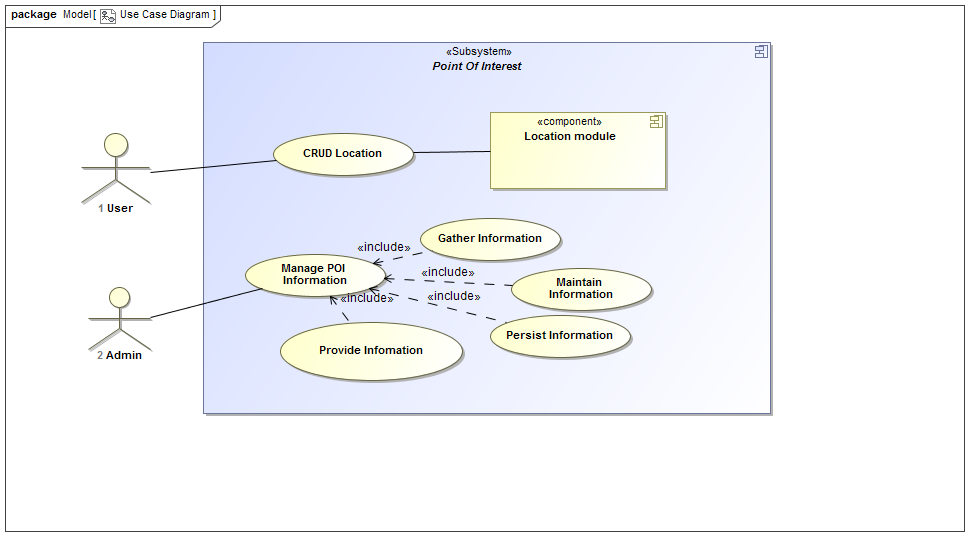
\includegraphics[scale=0.5]{Use_Case_Diagram.png}
 						\caption{Point of Interest Module Use Case Diagram}
 					\end{figure}
 				\end{center}
			
			\item Sequence Diagram
			\begin{center}
				\begin{figure}[!h]
					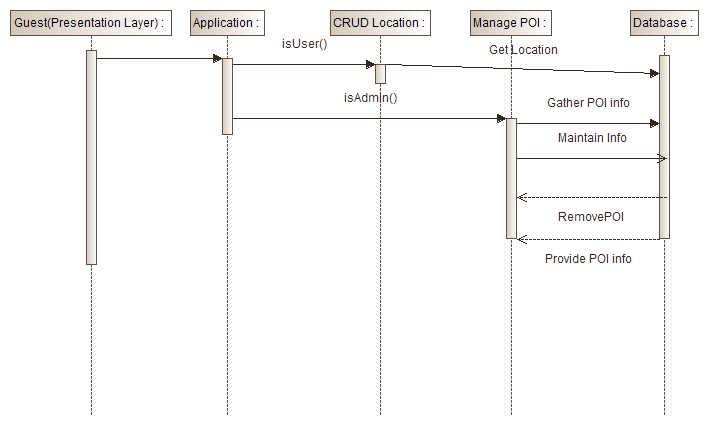
\includegraphics[scale=0.6]{POI_Sequence_diagram.png}
					\caption{Point of Interest Module Sequence Diagram}
				\end{figure}
			\end{center}
			\pagebreak
			
				\item Activity Diagram
 				\begin{center}
 					\begin{figure}[!h]
 						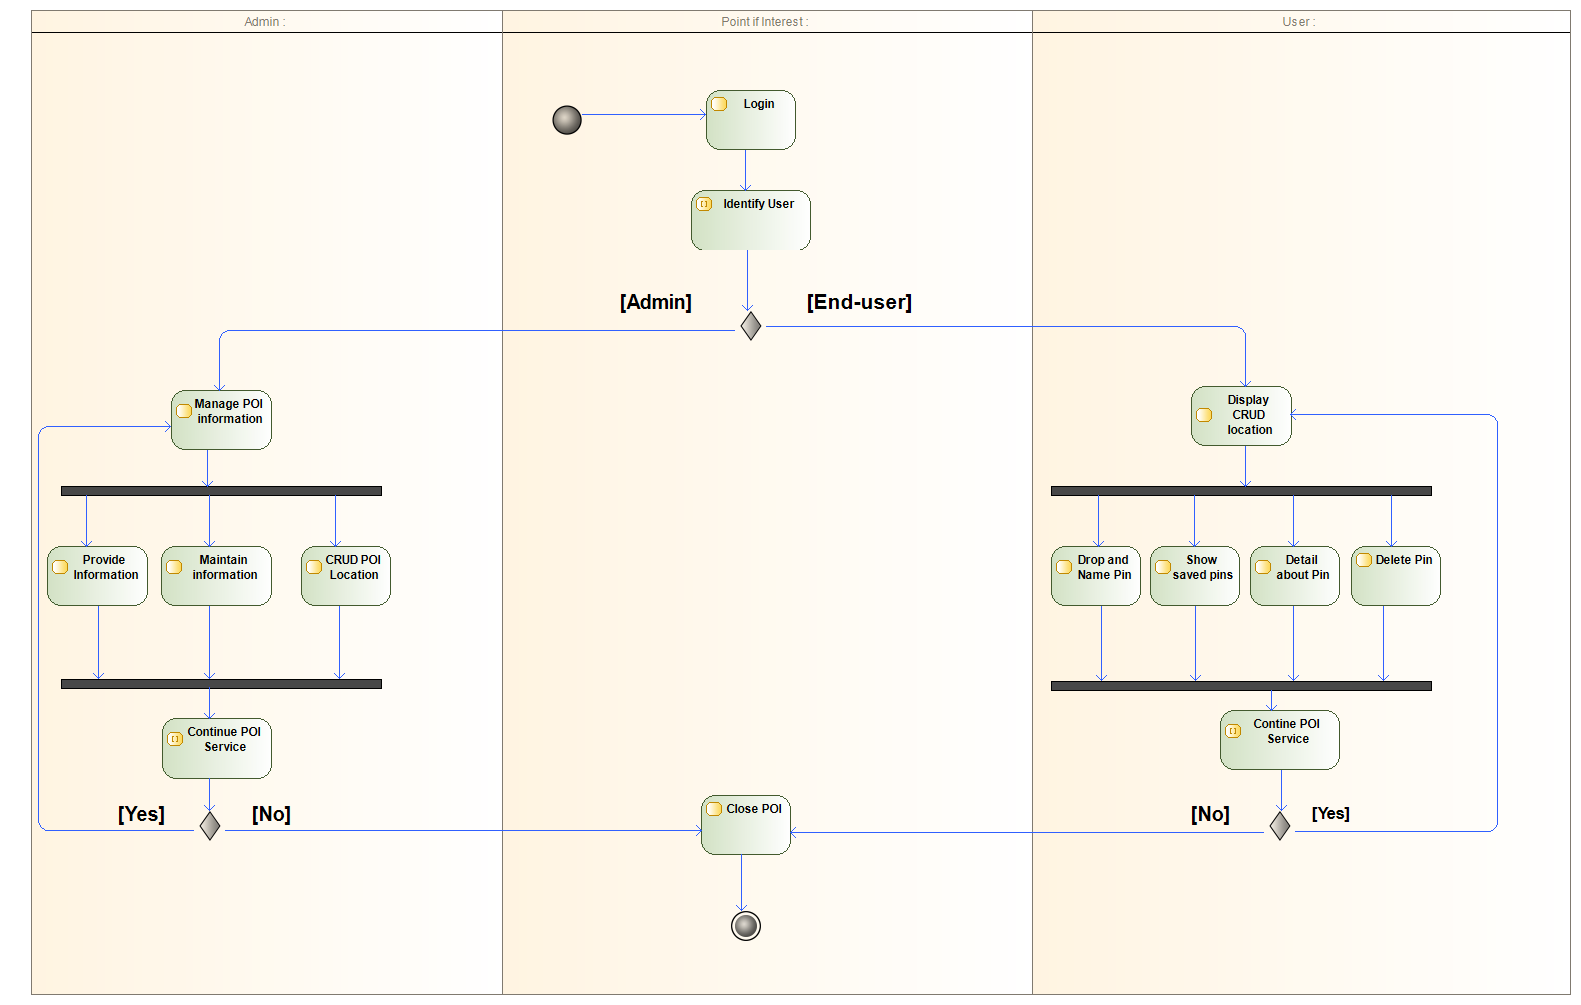
\includegraphics[angle=90, scale=0.375]{POI_Activity_Diagram.png}
 						\caption{Point of Interest Module Activity Diagram}
 					\end{figure}
 				\end{center}
 				\pagebreak
 				
 				\item State Diagram
 				\begin{center}
 					\begin{figure}[!h]
 						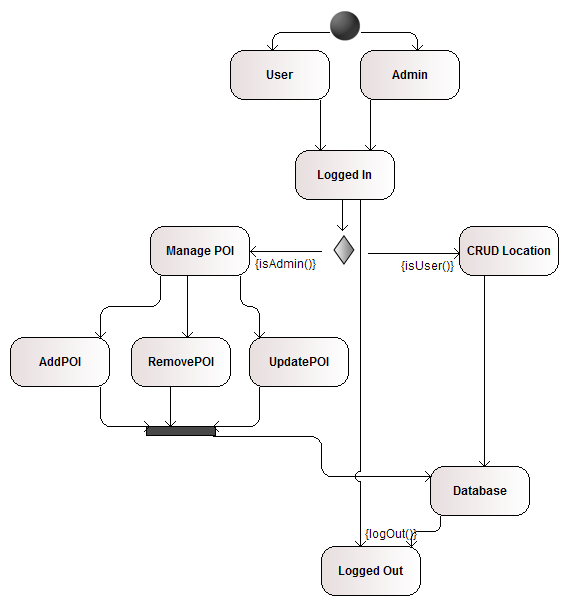
\includegraphics[scale=0.6]{POI_State_Machine_diagram.png}
 						\caption{Point of Interest Module State Diagram}
 					\end{figure}
 				\end{center}
				
				
			\end{itemize}
		\subsection{Events Subsystem}
		\subsubsection{Type of System and Architecture Design}
				In the case of the Events subsystem, we thought it would be relevent to use the "Observer" design pattern. This would allow for an efficient use of real time systems and help the process of updateing information about events immensly. This should streamline the process behind updating the Events fedd as well as providing the infomation to a multitude of users. 
				
			\subsubsection{External Interface Requirements}
					The external requirements for the Events module will boil down to the actual organisation of events and how the entire subsystem will be structured around real time updating of the application to provide information about a particular event as soon as possible. We would have to implement some for of push notification API in order to effectively update the events module and provide this kind of information.

			\subsubsection{Performance Requirements}
					Seeing as how most of this specific module will be about transfering information in real time, it would require that the systems in which it will be used will need to have some form of push API. Fortunately, most smartphones in this day and age will cater to that. Data and internet connection will be requirements for this modulae to work, you would not have to be connected to campus wi-fi as it would just be updating a feed of events happening in and around campus.
		
			\subsubsection{Design Constraints}
					This comes down to how the system will be updated. It should be noted that in order to keep the information about events precise, one admin user should take up the role of updating the feed. This means that we will end up having only one information source about these events. Further more, the design of the feed will have to be done in such a way as to nnot clutter the main interface and to take up as little space as possible in order to allow for more inmportant feature, such as navigation, to be more prominent.

			\subsubsection{Technologies}
				\begin{itemize}
				\item	RSS
				An rss feed type system wold be worth looking into as a means to distribute the information given to multiple users, it would allow a seamless transition to the presentation layer
				\item Presentation Layer
				Like with the User module, android studio would be used as well as other tech nologies for iOS. These along with RSS can be used to effectively craft a visually pleasing experience.

				\item Service Layer
				We will make use of the REST API for this module since its what we will be using for our other modules, this will allow us to easily communicate between modules as well as add additional functionality. We would also make use of ATOM for our RSS API. This would allow us to handle our information distribution across multiple users more efficiently.

				\item Business Layer
				This is where we implement all the logical technologies that add the functionality to this module. We shall be using JAVA to help the process of creating this module and streamlining the functionality between the different layers
				\end{itemize}
			
			\subsubsection{Design of Architecture}
				\begin{itemize}
					\item Class Diagram
					\begin{center}
						\begin{figure}[!h]
							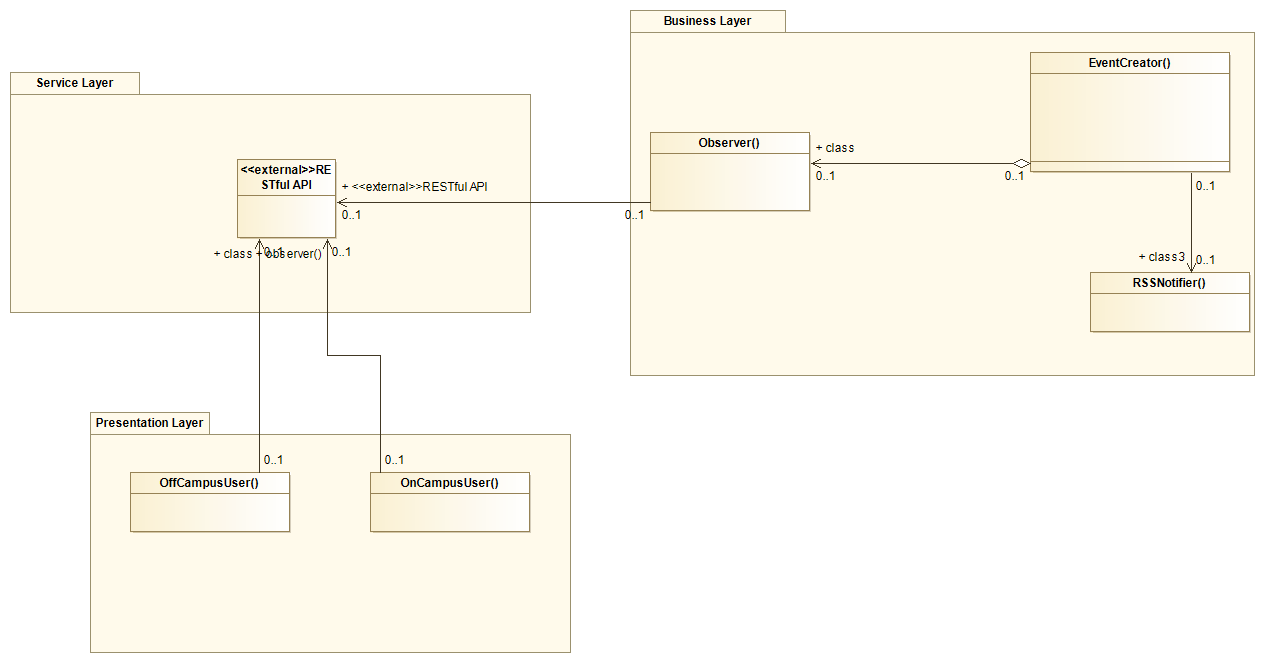
\includegraphics[scale=0.3]{Events_Class_Diagram.png}
							\caption{Events Module Class Diagram}
						\end{figure}
					\end{center}
					
					\item Deployment Diagram				
					\begin{center}
						\begin{figure}[!h]
							%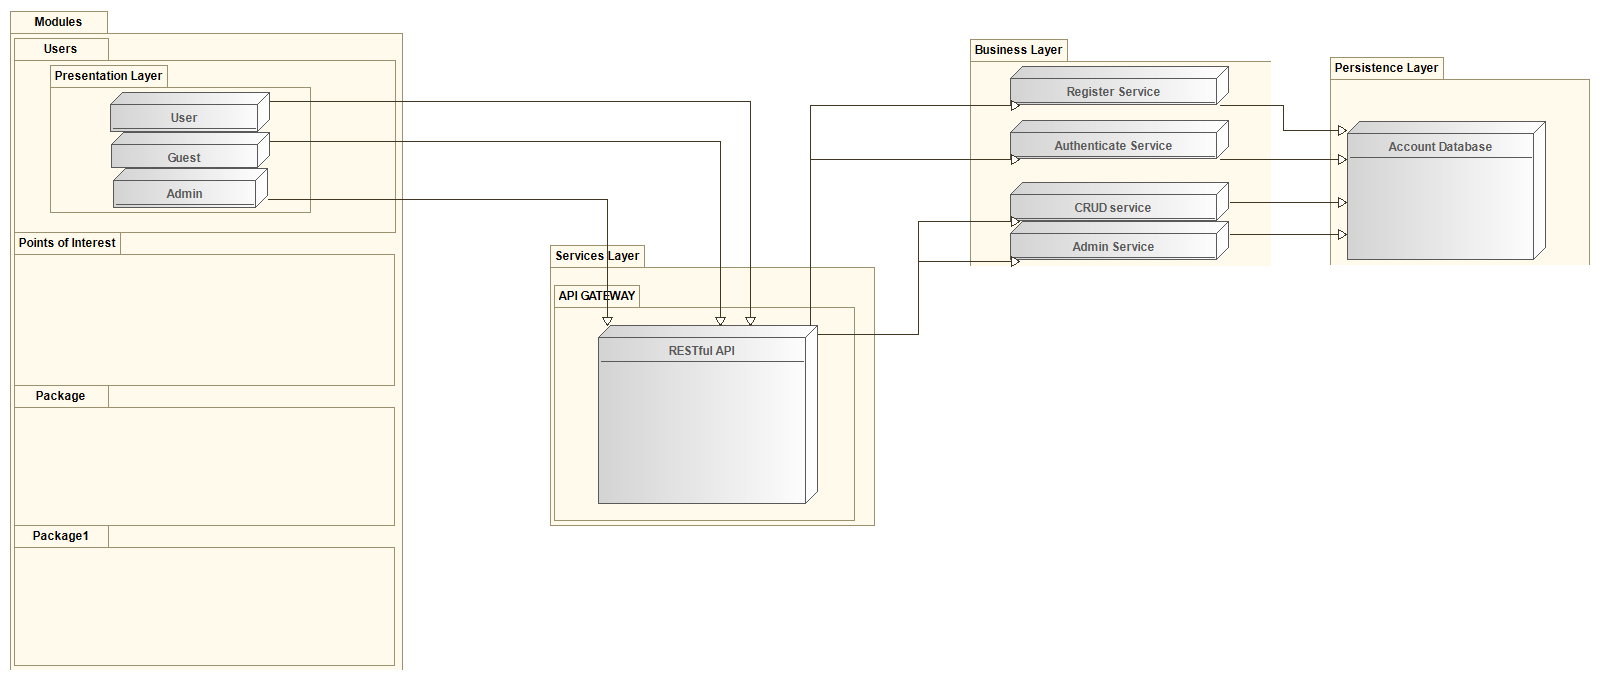
\includegraphics[scale=0.3]{dd.png}
							\caption{Events Module Deployment Diagram}
						\end{figure}
					\end{center}
					
					\item Use Case Diagram
					\begin{center}
						\begin{figure}[!h]
							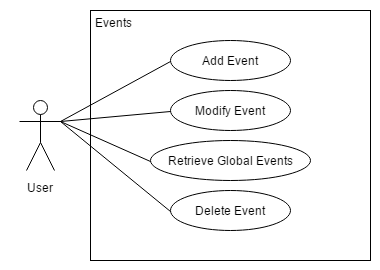
\includegraphics[scale=0.6]{Events_Use_Case_Diagram.png}
							\caption{Events Module Use Case Diagram}
						\end{figure}
					\end{center}
					
					\item Activity Diagram
					\begin{center}
						\begin{figure}[!h]
							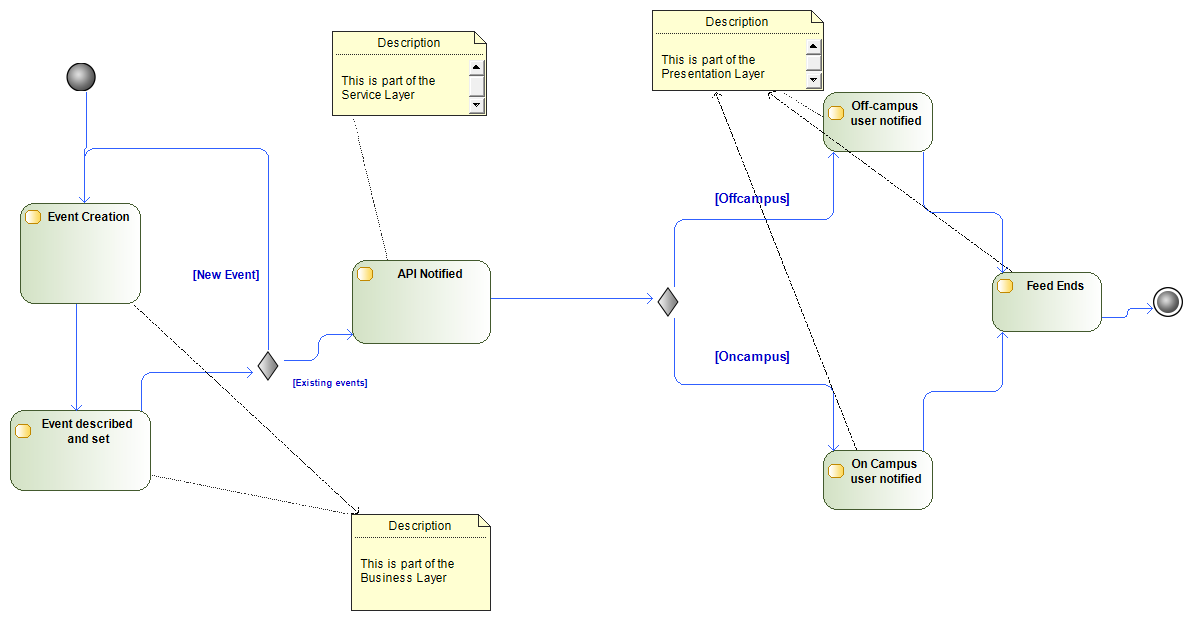
\includegraphics[scale=0.4]{Events_Activity_Diagram.png}
							\caption{Events Module Activity Diagram}
						\end{figure}
					\end{center}
										
				\end{itemize}
			
\end{document}
